\documentclass[10pt]{article}

% Page layout
\usepackage[margin=1in]{geometry}
\usepackage{setspace}
\usepackage{parskip} % No indent, space between paragraphs

% Fonts
\usepackage{mathptmx} % Times New Roman equivalent for math and text
\usepackage[T1]{fontenc}
\usepackage[utf8]{inputenc}

% Line spacing
\renewcommand{\baselinestretch}{1.5}

% Figures
\usepackage{graphicx}
\usepackage[labelfont=bf, labelsep=period]{caption}
\usepackage{float} % For [H] specifier

% Section formatting
\usepackage{titlesec}
\titleformat{\section}{\normalfont\Large\bfseries}{\thesection.}{0.5em}{}
\titleformat{\subsection}{\normalfont\large\bfseries}{\thesubsection.}{0.5em}{}

% Bibliography (basic)
% \usepackage[superscript,sort&compress]{natbib}

% Title
\title{\bfseries Using Monte Carlo Tree Search and Neural Networks in an AI Agent to Play Quoridor}
\author{
    Iram Liu, Jacob Groner, Mason Raffo
}
\date{May 17, 2025}

\begin{document}

\maketitle

\begin{abstract}
We present a Monte Carlo Tree Search and neural network evaluation method to play Quoridor, a two person deterministic strategy game with a high branching factor and numerous intricacies.
\end{abstract}

\section{Introduction}
Quoridor is a deterministic, two player game with perfect information. Each player has a pawn on a square board and a limited number of fences. Players start on opposing sides of the board, and their goal is simple: to reach their opponent's back row. On each turn, they may either opt to move their pawn a single space or to place a fence. Fences sit between board spaces and block pawns from moving across. Players are required to leave at least one viable path for their opponent to reach the goal, and the first player to reach their corresponding goal area wins the game.

\section{Project Description}

We sought to make an AI agent that was capable of playing Quoridor. Initially, we intended to focus on a primarily convolutional neural network-based approach and evaluate it against an agent that played using random roll-outs. As we progressed, we found that using random roll-outs presented significant challenges, eventually abandoning their use altogether. We implemented our preliminary attempts in python, but the language's high overhead forced us to complete our final implementations in C++. This reimplementation proved to be unexpecedtly difficult, costing us considerable time debugging the many edge cases surrounding pawn moves.

After our networks were complete, we found that the convolutional neural network was under-performing. We investigated deeper into the mechanics of the game, and outsourced some complex pathfinding logic to features before the network. Our second network had fewer parameters, but performed better due to the computations encoded in its input features.

\subsection{Rules of Quoridor}

As previously discussed, Quoridor is played on a square board and each player controls one pawn (Fig.~\ref{fig:rules}A). Quoridor has several variations, and many of them use a $9 \times 9$ sized board. We have opted to use a $5 \times 5$ board due to limited computing resources. The aim of the game is to move your pawn into the goal regions (Fig.~\ref{fig:rules}C). To slow down their opponent, players have a certain number of fences that they may place on the board to block their opponent's path. These fences each span two spaces, and player cannot cross a fence (Fig.~\ref{fig:rules}B). A fence may not be placed if doing so would block either player's only remaining path to the goal (Fig.~\ref{fig:rules}D). Pawns may never occupy the same space. To prevent stalemates, pawns may jump over each other if their path is blocked (Fig.~\ref{fig:rules}E). Pawns may jump diagonally only if a fence blocks their primary jump (Fig.~\ref{fig:rules}F). To limit the length of games, we instituted a move limit. Games that exceed this number of moves are declared to be drawn.

\begin{figure}[H]
    \centering
    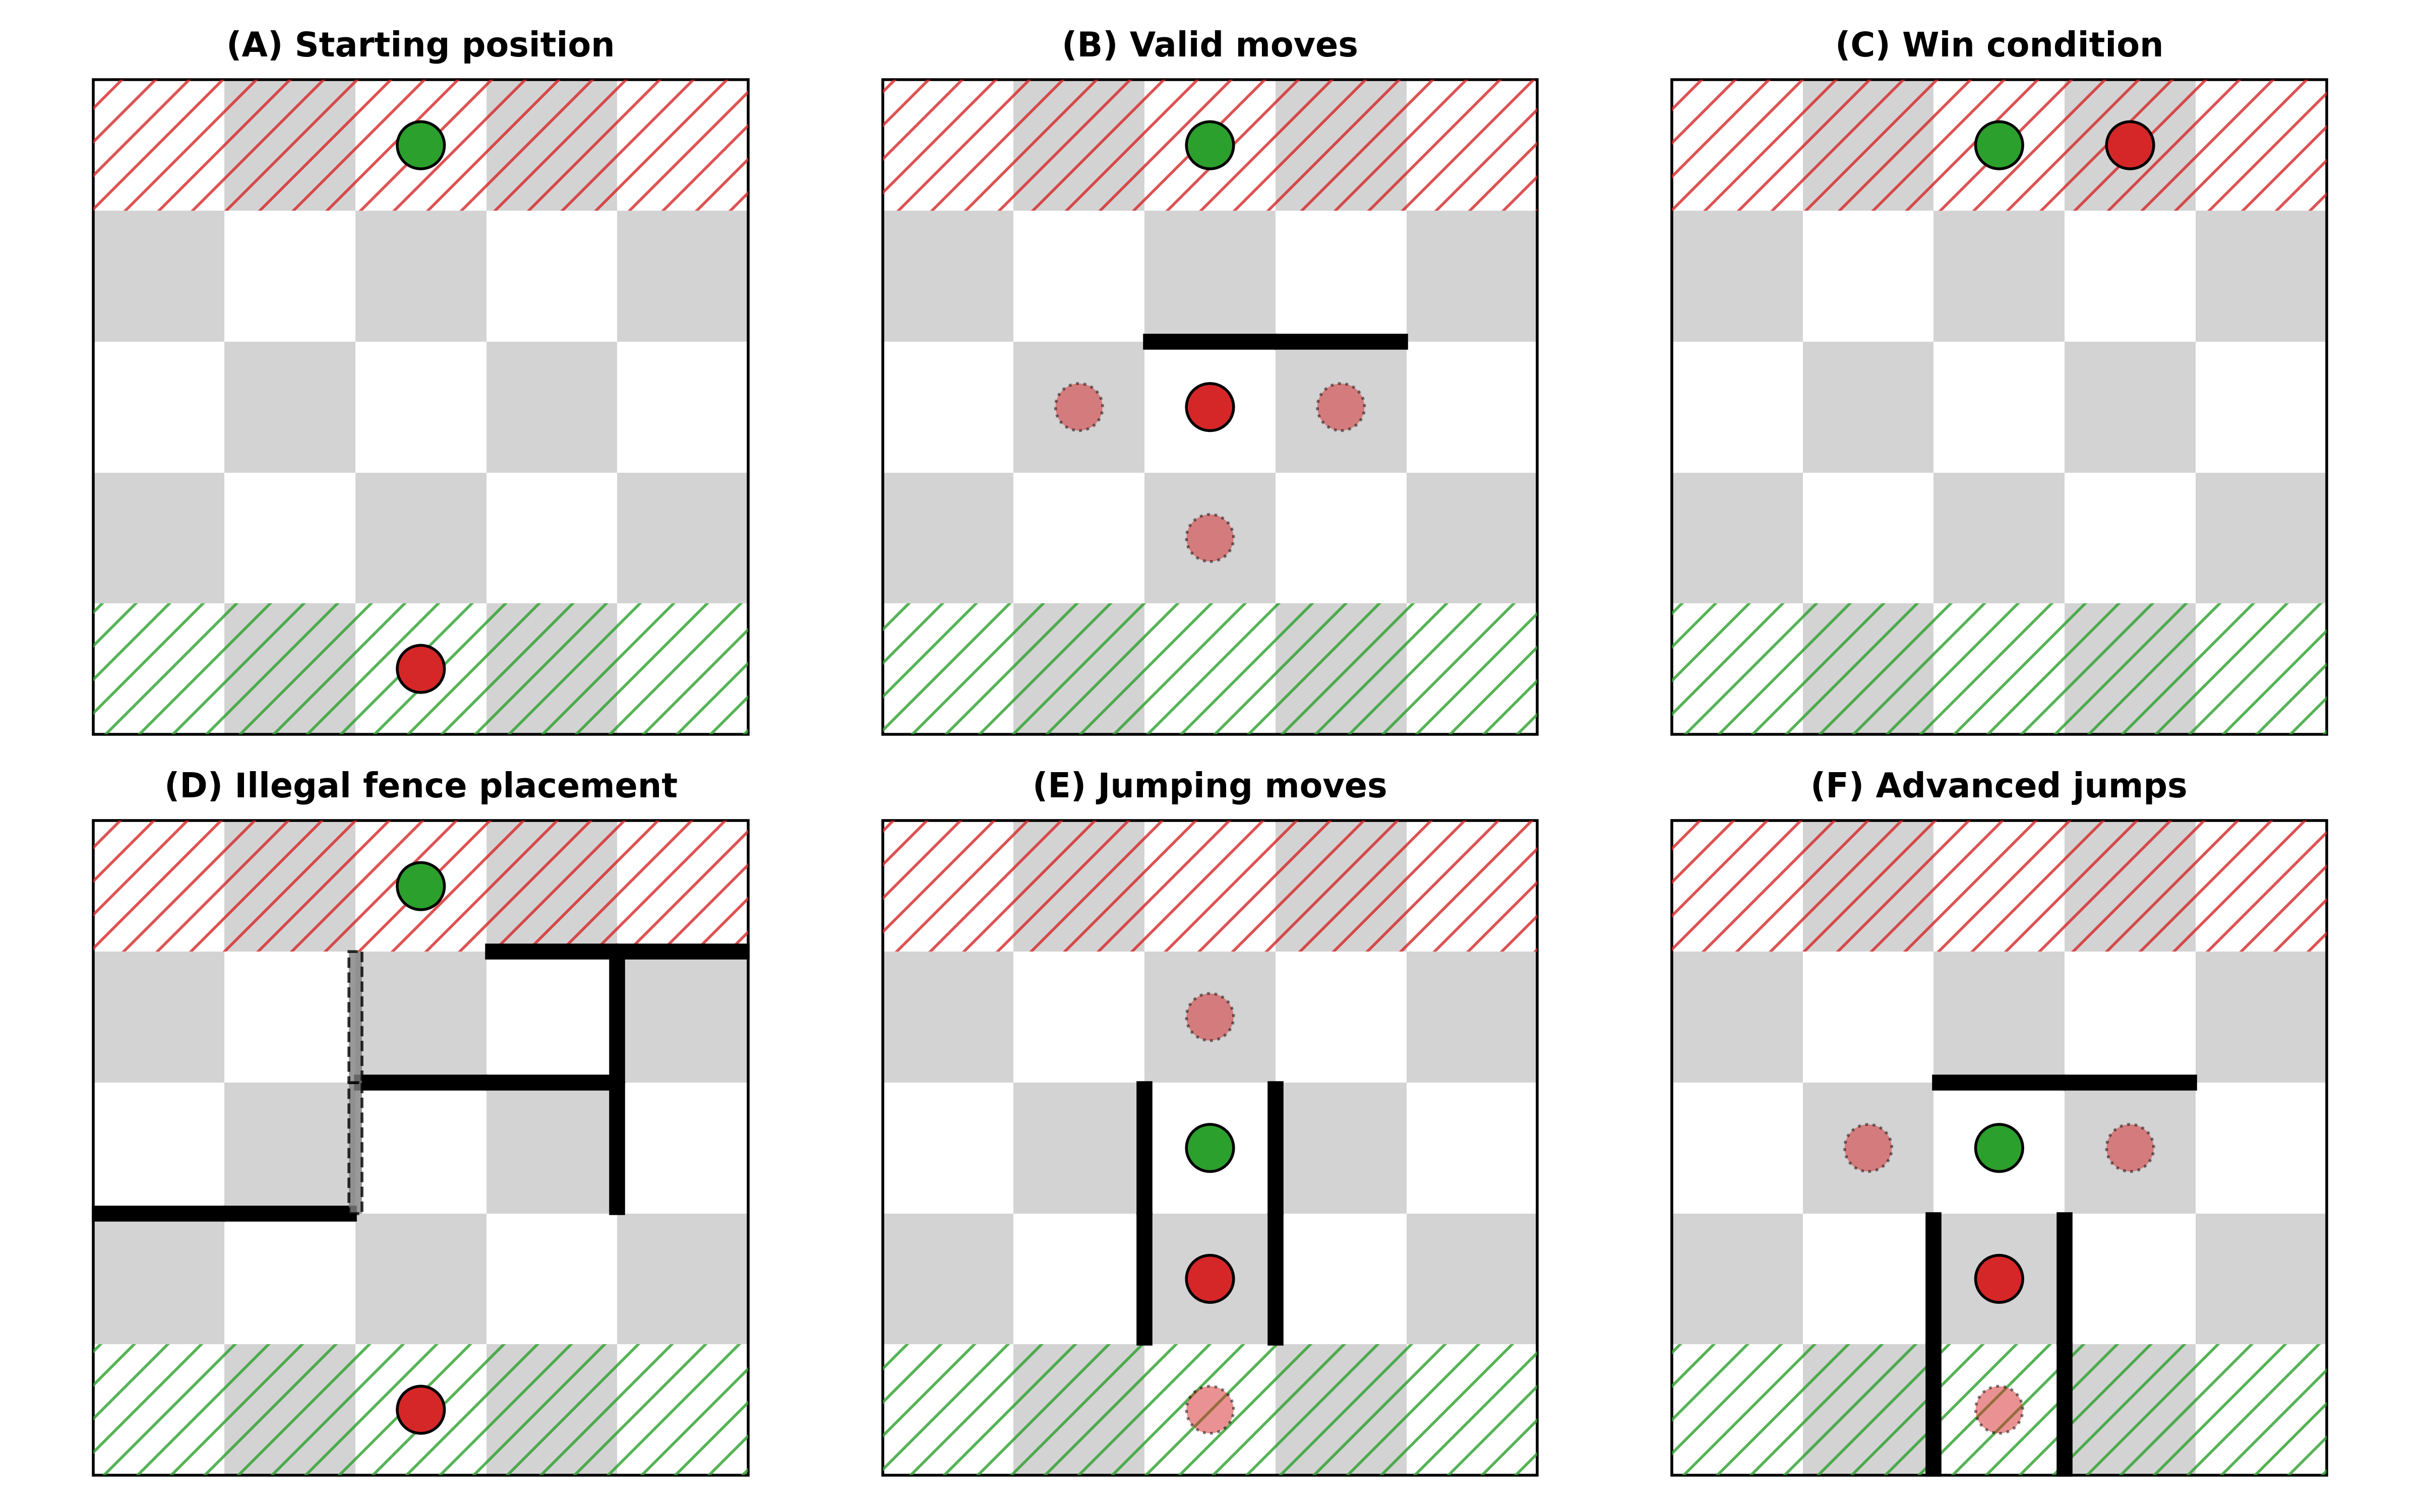
\includegraphics[width=\linewidth]{rules_demo.png}
    \caption{\textbf{Rules illustrations.} \textbf{(A)} The starting position. Player 1 is red; Player 2 is green; Fences are black lines. Hashed regions denote the goal area a player must reach to win. \textbf{(B)} Valid pawn moves for player 1 are shown. \textbf{(C)} Player 1 has won the game. \textbf{(D)} Fences cannot be placed if they completely block either player from reaching the goal area. The lightly shaded fence would not be allowed. \textbf{(E)} If a player is blocked by the opposing pawn, they may jump over. \textbf{(F)} Pawns may move diagonally only if a fence blocks a player's jump.}
    \label{fig:rules}
\end{figure}


\subsection{Monte Carlo Tree Search}

In principle, Quoridor could be a solved game. However, each position has a staggering number of possible moves which makes a brute force tree search infeasible. The multitude of interacting ``pawn jump'' moves makes a case analysis proof impractically complicated. Instead, we present an AI agent to play the game using a Monte Carlo Tree Search (MCTS) and a neural network based game state evaluation method.

\textbf{Citation needed for MCTS}

MCTS is a method of evaluating and iteratively expanding a game tree, the tree of all possible moves from a given position. In an environment where exploring every possibility is impossible, this process aims to balance two competing philosophies of position analysis: exploration and exploitation. Exploration involves devoting time to expanding less-searched areas of the game tree. While the initial analysis indicated that these potential moves had little value, it is possible that there are intricacies that make them extremely valuable moves with the right follow-up strategy. Exploration is about finding these hidden moves.

Exploitation, on the other hand, focuses on more deeply expanding a few promising ideas. The first layers of analysis indicate that these moves are encouraging, and a deeper analysis could determine which is the absolute best. With limited computing time and resources, it is impossible to fully explore both exploration and exploitation. MCTS provides a method to find an equilibrium between devoting all the resources to one or the other.

MCTS is performed iteratively. The primary data structure is a tree, with nodes that represent possible game states and edges that represent a possible move. The children of a node are all the possible moves that a player could make given the current position. The root of the tree represents the current game state. A leaf node either represents a terminal state (the game is over) or an unexplored possibility. An iteration of the MCTS expands one leaf node of the tree to consider one more move into the future along that branch of play. Each iteration has four phases: selection, expansion, evaluation, and backpropagation.

\subsubsection{Selection}

\textbf{ADD CITTAION FOR FORMULA}

The selection phase is key in the MCTS's ability to balance exploration with exploitation. During the selection phase, the algorithm decides which leaf node in the game tree to expand. Starting from the root node, children nodes are recursively selected until a leaf node is reached. Children are scored with the following expression, and the child with the highest score is selected.

\begin{equation}
    \frac{w}{n} + c \sqrt{ \frac{\ln N}{n} }
\end{equation}

In this expression:

\begin{itemize}
    \item $w$ is the sum of evaluations for this node and all of its children.
    \item $n$ is the number of times this node has been selected.
    \item $N$ is the number of times this node's parent has been selected. 
    \item $c$ is the exploration parameter. Higher values will prioritize exploration while lower values will emphasize exploitation.
\end{itemize}

Empirical testing and analysis is usually necessary to select an appropriate value for $c$. If there are any child nodes that are yet to be selected ($n = 0$), one of them will always be selected to avoid divide by zero errors.

\subsubsection{Expansion}

If the selected node is a terminal state (the game is won, lost, or drawn), this step is skipped. Otherwise, the selected leaf node is expanded. Every possible move from the game state represented in the selected node is added as a child to the leaf node.

\subsubsection{Evaluation}

Perform an evaluation for the selected node. This step will vary based on the method in use. In general, the evaluation function $f$ is a scalar valued function that maps a game state to an evaluation value $e$ such that $-1 \leq e \leq 1$. Terminal states are always mapped to one of $\{1, -1, 0\}$ depending on the outcome. A good evaluation function would map game states that are more favorable to the current player as higher values, less favorable game states to lower values. 

\subsubsection{Backpropagation}

After the evaluation is determined, it is recursively backpropagated to every parent node. Concretely, the value of $w$ is updated for every node such that $w \gets w + e$. The evaluation is then flipped with the operation $e \gets -e$ and passed to the current node's parent. The evaluation must be flipped because the evaluation is always from the perspetive of the player to move, so a strong position for a child is a weak position for its parent. This processes is repeated until the root node is reached.

\subsection{Heuristics}

If a game tree can be fully expanded, one can use trivial algorithms to determine which player can force a win. (The Minimax decision rule is one example.\textbf{CITATION HERE}) When the game tree cannot be fully expanded, it is necessary to create a heuristic that can determine the value of a position. The accuracy of the heuristic function is directly correlated with the playing strength of the AI agent. A perfect heuristic that could always determine which player has forced win would lead to an optimal AI agent. In this project, we compare five distinct heuristic methods:

\begin{enumerate}
    \item \textbf{Random roll-outs.} Moves are played randomly until one player wins. The evaluation corresponds to the winning player.
    \item \textbf{Naive.} Has no knowledge of the game at all. Always gives a neural evaluation unless a player has successfully won the game. Serves as a baseline for comparison.
    \item \textbf{Basic.} Gives a basic scaled value based on the Manhattan distance to the goal. Does not take any pathfinding or advanced logic into account.
    \item \textbf{Convolutional Neural Network.} Uses a convolutional neural network that analyses the board position.
    \item \textbf{Path Resiliency Neural Network.} Uses an MLP that has advanced knowledge of potential paths to the goal encoded as features.
\end{enumerate}

\subsection{Convolutional Neural Network Design}

\subsection{Shortest Path Resiliency}

The player with the shortest path to the goal will win without intervention by their opponent. The primary intervention is fences, which can be placed to block the previously existing shortest path between a player and the goal region. However, determining the ideal placement of fences is not trivial. Some placements will force a longer detour than others, and some placements will impede the player placing them more than their opponent. We created the resiliency method to provide our neural network with insight into the  impact fence placements will have on the outcome of a given game position.

This technique aims to find ``bottlenecks,'' or fence placements that will optimally disrupt the opponent while providing minimal disruption to the current player's path. In doing so, the model will be able to determine how resilient a player's path to the goal is. Paths with high resiliency are difficult to disrupt with fence placements. Paths with low resiliency may be shorter in absolute distance, but they are easily made much longer by a few well-chosen fences.

This technique takes the board position and constructs a graph with each board space represented as a node. Path resiliency is calculated independently for each player. Weighted, undirected edges are added between adjacent board positions that are not separated by a fence. These represent valid pawn moves. Each edge is initialized to the same starting weight $w_{init}$.
(For pathfinding simplicity, there is final node that is connected to all of the nodes in the goal area by an edge of weight 0. Pathfinding algorithms can target this node, and in doing so, find an optimal path to any part of the goal area.) % TODO: Move this to a figure caption somehow? It's too wordy for the main paragraph
Then, a two step iterative process begins:

\begin{enumerate}
    \item Calculate the shortest weighted path $P$ from the target player to the goal region. (Use Dijkstra's algorithm or an equivalent.)
    \item Add an amount $\delta$ to every edge along $P$.
\end{enumerate}

This technique shines when there are many paths to the goal for both players, and these paths may overlap (Fig.~\ref{fig:resiliency}A). After several iterations, edges that are difficult to avoid will accumulate extreme weight values, and edges that have equivalent alternate routes will have the additional weight distributed amongst them (Fig.~\ref{fig:resiliency}B-C). Edges with high weights are good targets for fence placements. However, fences block the player placing them as well as their opponent. We aim to encode the viability of blocking an edge by subtracting the resiliency weights of the current player from the opponents (Fig.~\ref{fig:resiliency}D).

\begin{figure}[H]
    \centering
    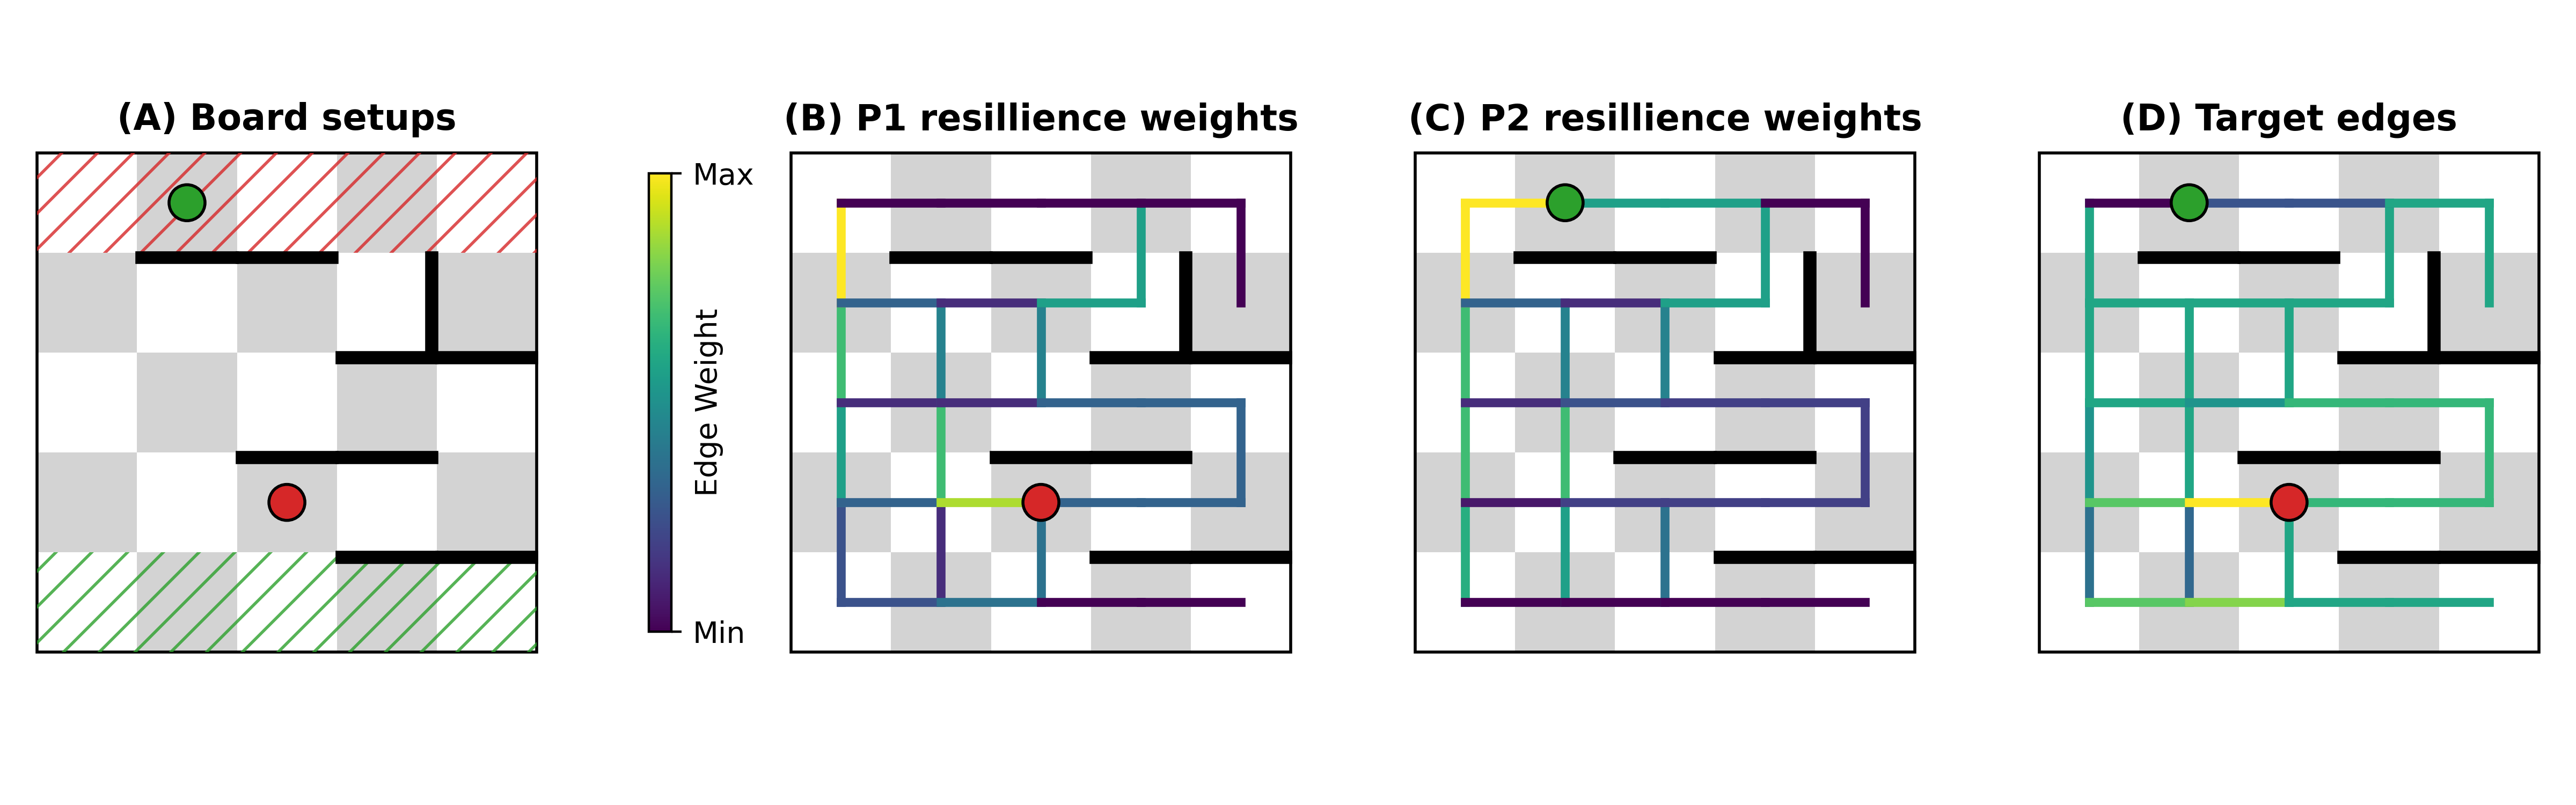
\includegraphics[width=\linewidth]{path_figure.png}
    \caption{\textbf{Path resiliency.} \textbf{(A)} An example position of the board. Player 1 is red; Player 2 is green; Fences are black lines. Hashed regions denote the goal area a player must reach to win. \textbf{(B, C)} Resiliency weights of players 1 and 2, respectively. Higher values indicate that the edge is harder to avoid when finding alternative short paths to the goal area. \textbf{(D)} Calculated as player 1 resiliency weights minus player 2 resiliency weights. A high values indicates that the edge is very damaging to player 1 when blocked, while not damaging to player 2. In this example, a fence placed directly to the left of player 1 would require major detours for player 1 without interrupting many of player 2's paths to the goal. Thus, it has a high weight.}
    \label{fig:resiliency}
\end{figure}

Due to the discrete and uniform nature of these edge weight modifications, the number of iterations is not relevant beyond a sufficient threshold ($=25$, in our testing). After sufficient iterations, all the resulting weights are nearly equivalent up to scale.

There are several features we create for our neural network using this process. Each feature is calculated twice: once from each player's perspective.

\begin{enumerate}
    \item \textbf{Scaled resiliency distance.} This scalar encodes the information of Fig.~\ref{fig:resiliency}B. It is the percentage of the total weight that is included in the shortest path from the player to the goal after all of the iterations are complete.
    \item \textbf{Raw resiliency distance.} This scalar is similar to (1), but it does not depend on the amount of total weight added during the iterative phase. It is calculated as the total weight along the shortest path to the goal divided by the number of iterations.
    \item \textbf{Scaled targetability.} This scalar encodes the information of Fig.~\ref{fig:resiliency}D in the same method as (1).
    \item \textbf{Raw targetability.} This scalar encodes the information of Fig.~\ref{fig:resiliency}D in the same method as (2).
    \item \textbf{Maximum liability.} This scalar encodes the intensity of the highest weight of Fig.~\ref{fig:resiliency}D.
\end{enumerate}

\subsection{Training Data Generation}

\section{Evaluation}

\subsection{Principles of Evaluation}

As noted earlier, the strength of an MCTS system is entirely dependent on the strength of its evaluation function, the number of search iterations it performs, and the proper balance between exploration and exploitation. To confirm that our MCTS system was working as expected, we conducted several tests. These tests aim to validate the performance of our system by checking for two principles:

\begin{enumerate}
    \item As the number of iterations is increased for a given system, the playing strength should increase.
    \item As the accuracy of the evaluation function improves, the number of iterations that are required to achieve the same level of performance should decrease.
\end{enumerate}

The first principle verifies that an MCTS system is working as expected, while the second principle gives us a method of comparison between different systems.

\subsection{Principle 1: Increasing Iterations Improves Performance}

To verify that increasing the number of iterations increased the performance of our models, we created a methodology to determine the relative playing strength between two models. A first thought would be to play the model against itself; however such a method would only test the model against positions that it itself selects rather than the full breadth of positions that it could encounter. Instead, we conduct many test games and begin each test game with a seqeuence of randomly selected moves. While this process does ensure the model is forced to play from a variety of unique positions, it presents a certain unfairness. Some positions are clearly lost, and are easily converted to wins by the opponent. We avoid this issue by looking at the ratio of wins to losses and draws. Stronger models will be able to find more subtle paths to victory, and will thus achieve a higher win to loss ratio against weaker models when starting from random positions.

\begin{figure}[H]
    \centering
    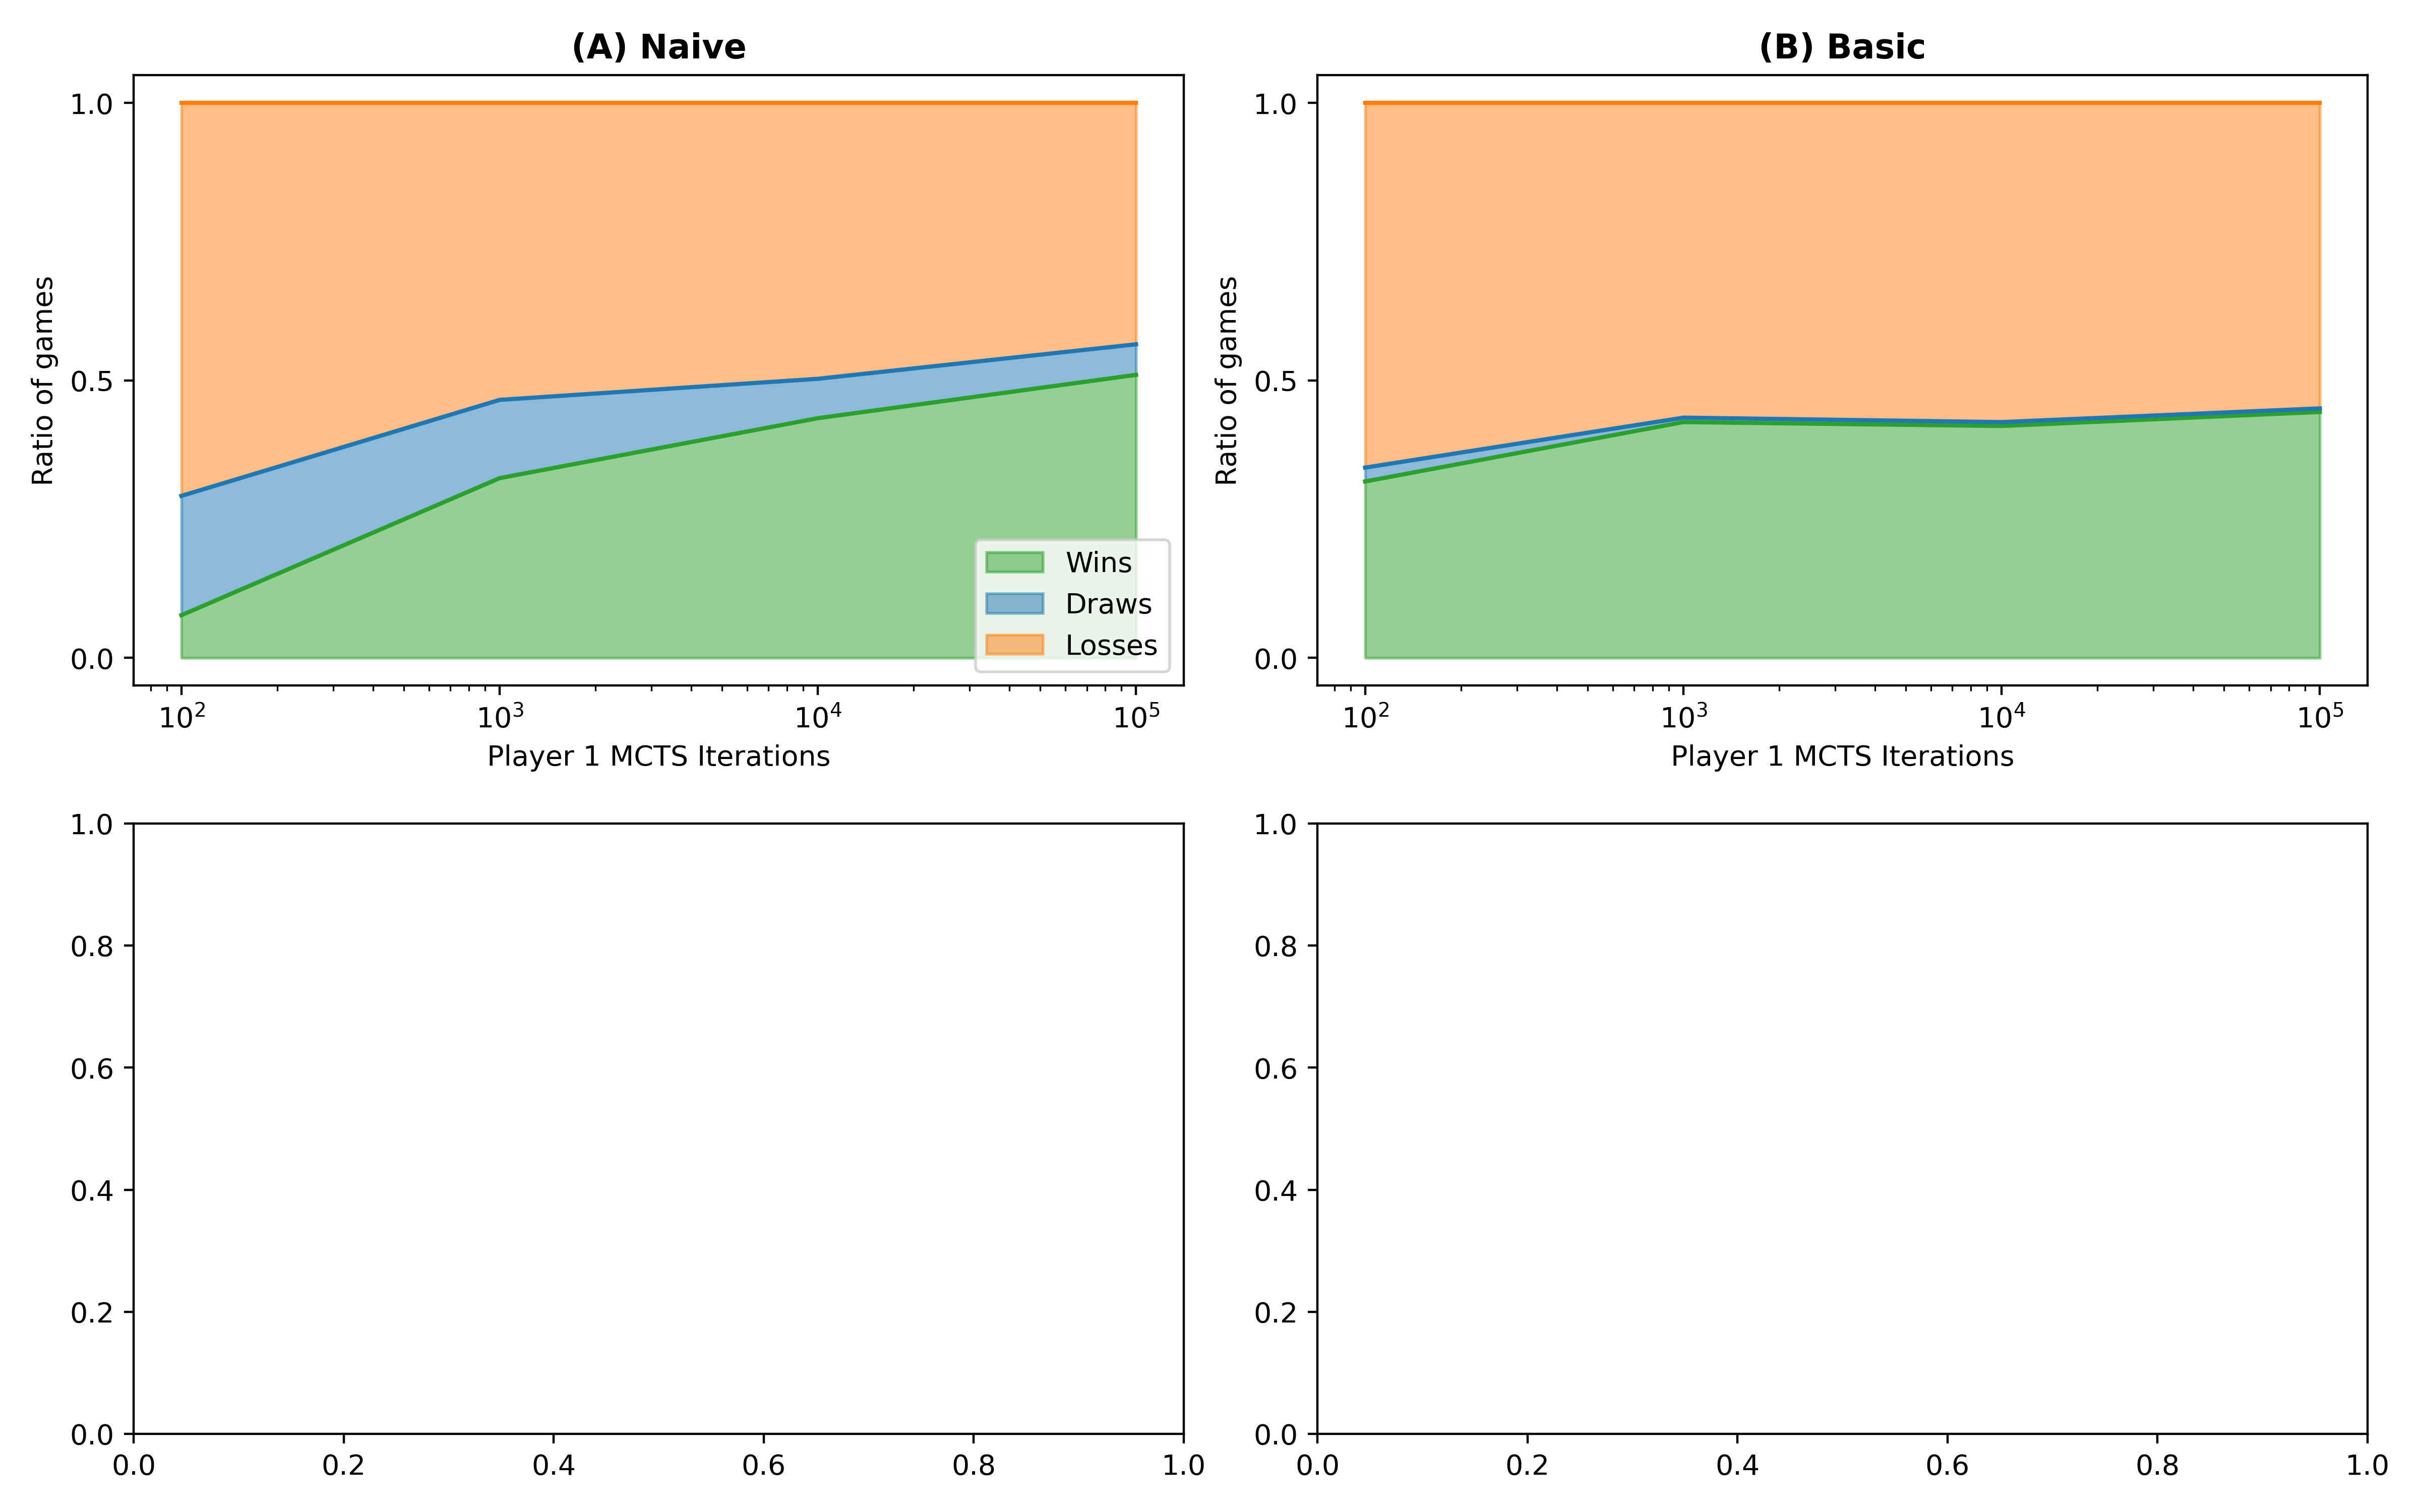
\includegraphics[width=\linewidth]{win_rates.png}
    \caption{\textbf{Self play.} All models play as player 1 against the naive MCTS model as player 2. The number of MCTS iterations for the model in question (player 1) varies. The number of iterations for the naive opponent (player 2) is constant ($= 1000$). Every game is started with 8 random moves (4 for each side). Random moves are drawn uniformly from the set of all legal moves.}
    \label{fig:selfplay}
\end{figure}

When playing the naive model against itself, our tests indicate that the performance increases as the number of iterations increases as expected (Fig.~\ref{fig:selfplay}A). Interestingly, when the number of iterations for both players are equal at 1000, player 2 wins. This potentially indicates that the game mechanics or the use of random moves biases towards player 2. Nevertheless, principle 1 is supported in this test.

When playing the basic model against the naive model, there is a similar upward trend (Fig.~\ref{fig:selfplay}B). The model also reaches a similiar peak performance, the point at which increasing the iterations does not provide performance enhancements. Although, the basic model reaches this peak performance at a lower number of iterations, supporting the theory that its evaluation function is more accurate. 

\subsection{Principle 2: Better Evaluations Functions Require Fewer Iterations}

MCTS systems compensate for imperfect evaluation functions by iteratively exploring and exploiting the most promising potential moves. As the number of iterations increases, the model's understanding of the position becomes more complete, and its analysis becomes more accurate. We compare several different evaluation functions to understand how quickly our models are able to understand more complex positions.

We have the models evaluate a prearranged position (Fig.~\ref{fig:MCTS}A). This position is designed like a tactics puzzle in chess: there is a clear winner with a bit of subtlety in the execution. First, we verify that our MCTS system is able to solve the puzzle. This puzzle is designed as a forced win for player 1, but there is only one right move. Every other move allows player 2 to force a win. The MCTS system selects the best move by finding the child of the root node with the highest $w / n$ ratio. We examine these ratios after 200 and 5000 iterations. It is clear that the model has found the best move after 200 iterations, and it is even more certain after 5000 iterations (Fig.~\ref{fig:MCTS}B).

We use the naive MCTS system as a baseline to compare other systems against. Its evaluation function provides no information about the board, only returning a nonzero value in terminal positions. When MCTS systems evalute with the naive evaluation function, there is an immediate and rapid drop (Fig.~\ref{fig:MCTS}D). This drop is an expected result when analyzing a position with a hidden tactic. With only a shallow search, it seems that the position is lost. It is only after the model has found the winning move and sufficiently explored to verify the expected outcome that the evaluation the increases. As expected, the calculated strength of the position continues to increase until the end of the experiment.



\begin{figure}[H]
    \centering
    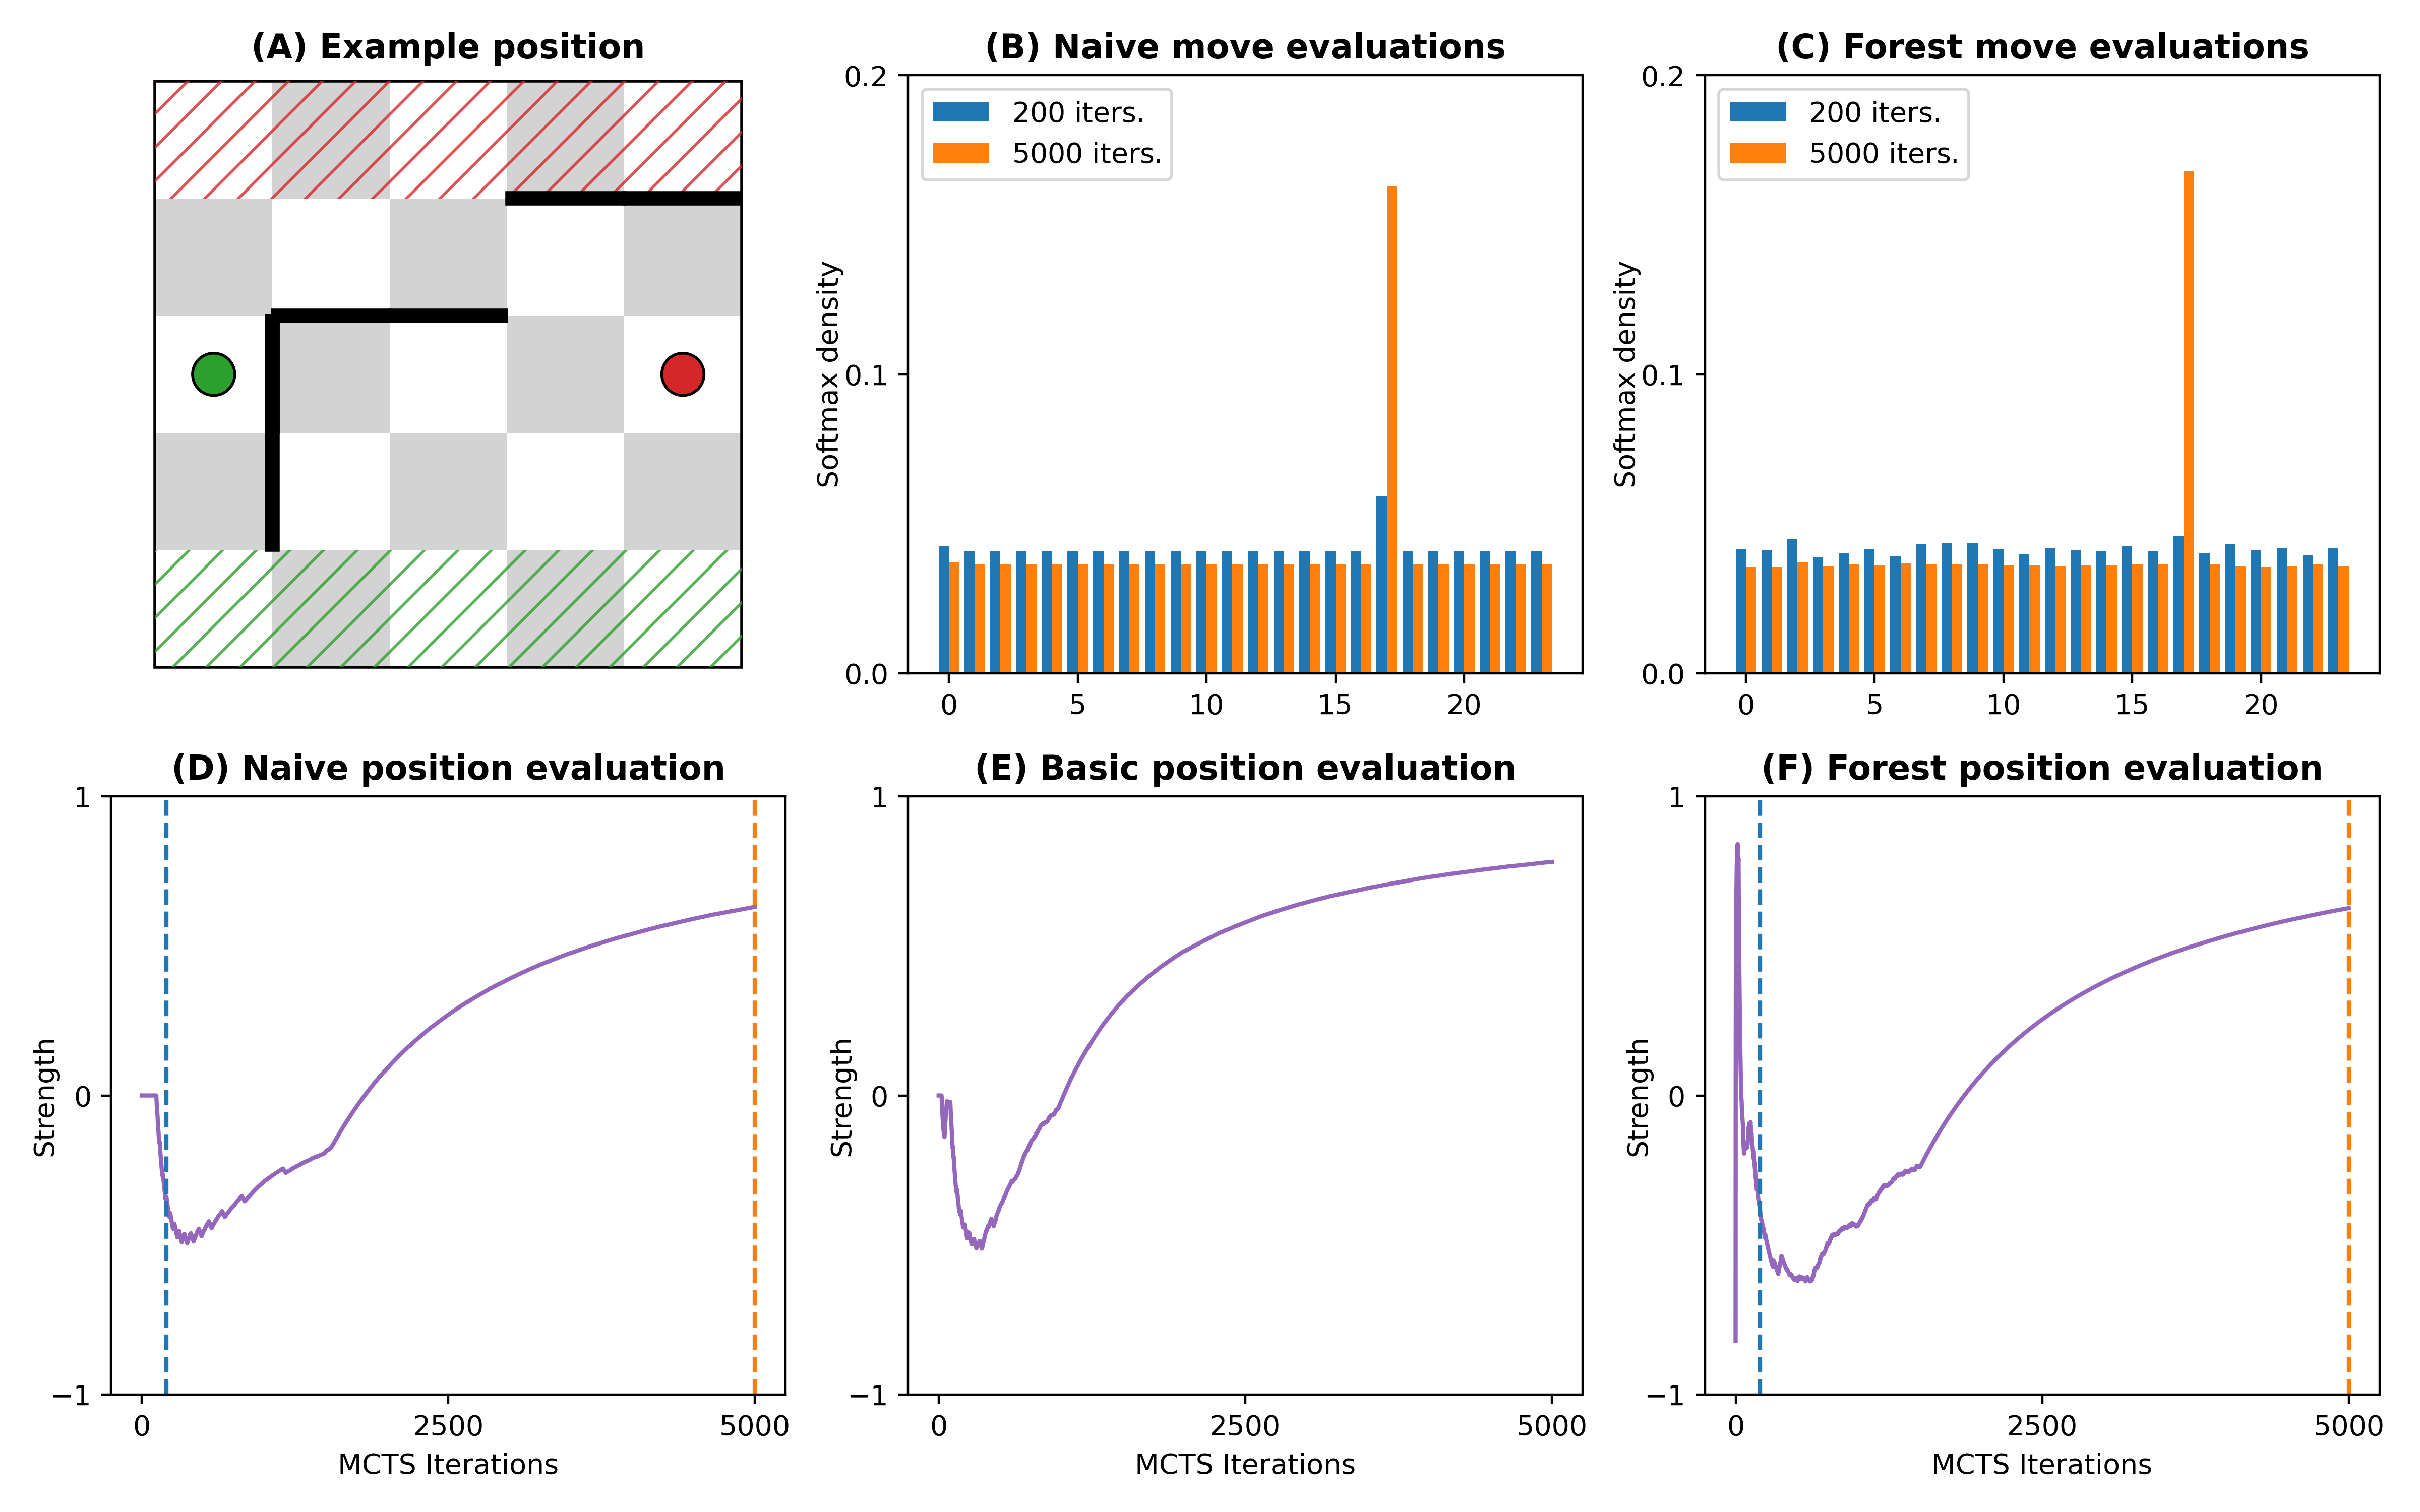
\includegraphics[width=\linewidth]{MCTS_eval.png}
    \caption{\textbf{Solving a Simple Tactic.} \textbf{(A)} A sample benchmark position that we selected to examine the model's strength as the iteration count increases. Player 1 (red) is to move. If they move directly toward the goal, they will lose and player 2 (green) will reach their goal first. However, if they block player 2 using a wall, they will win. For simplicity, each player has one wall remaining to place. This simple strategy puzzle should be solveable by all MCTS systems with enough iterations. \textbf{(B, C)} There are 24 valid moves from this position. Exactly one of them prevents player 2 from winning the game. This winning move is marked with *. This graph illustrates the softmax of $w/n$ for each possible move after 200 and 5000 MCTS iterations of the basic MCTS model. Higher bars indicate moves that the model prefers. \textbf{(D-F)} Various models' evaluations of the position as they perform more MCTS iterations. The correct evaluation is 1, as the position is  a forced win. Dashed lines indicate when the histograms were sampled.}
    \label{fig:MCTS}
\end{figure}

The basic evaluation function provides an iterative improvement over the naive function. Comparing the strength calculated by the basic evaluation function to the strength calculated by the naive evaluation function reveals a similar yet improved pattern (Fig.~\ref{fig:MCTS}E). There is a rapid drop followed by a more gradual improvement as the model gains understanding of the position. However, this model approaces the correct evaluation more quickly, confirming the improved performance of the evaluation function. 


\begin{figure}[H]
    \centering
    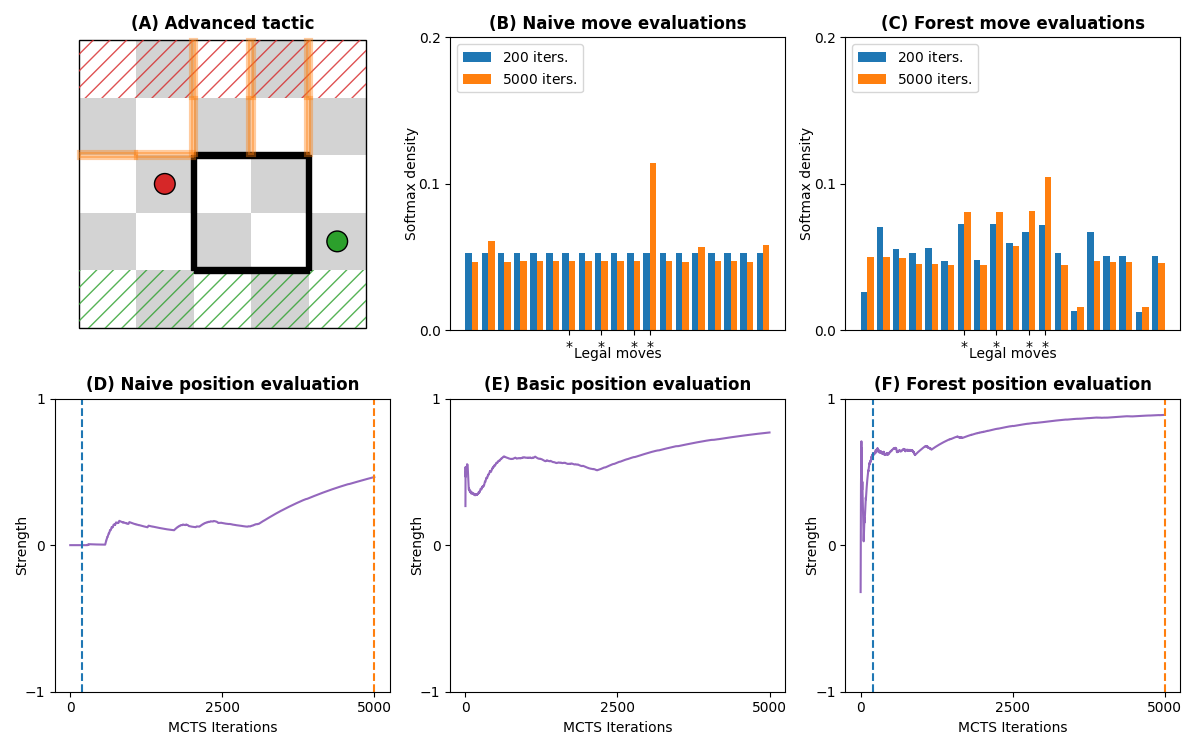
\includegraphics[width=\linewidth]{Adv_tactic.png}
    \caption{\textbf{Advanced Strategy.} \textbf{(A)} This puzzle is player 1 (red) to move. Each player has one fence remaining to place. Player 1 is closer to their goal and moves first, but they are susceptible to a fence blocking their path. If player 2 (green) is able to block player 1 with a fence, player 2 can force a win. Player 1 must employ an unintinitive move to maintain the lead: placing a fence to block their own unopportune paths to the goal. As the rules require that every player have a path to the goal, if a player delilberately blocks their own alternative paths, their opponent will not be allowed to block them with fences. There are four legal fence placements that player 1 employ to accomplish this goal. These placements are denoted as shaded orange boxes. These are the only winning moves for player 1. \textbf{(B-F)}~See Figure~\ref{fig:MCTS}.}
    \label{fig:AdvTactic}
\end{figure}

% \section{References}
% Cite your sources using \texttt{natbib} style: \cite{example}.

% \bibliographystyle{naturemag}
% \bibliography{references}

\end{document}

